\section{Resultados}

\subsection{Itemsets Frequênts}
\begin{frame}

    \frametitle{Resultados}

    \begin{itemize}
    
        \item Regionais Distantes do Centro
            \begin{itemize}
                \item Caracterizadas pela maioria de casas de padrões de acabamento entre um e três e lotes vagos;
                \item A Pampulha se destaca por ter casas de padrão 4 e não apresentar casas com acabamento padrão 1.
            \end{itemize}
            
        \item Regionais Vizinhas ao Centro
            \begin{itemize}
                \item Regionais Oeste e Nordeste predominam casas com padrão igual às regionais mais distantes;
                \item Leste e Noroeste possuem um padrão misto de casas, barracões, comércio local e lotes vagos, com padrões variando do 1 ao 3.
            \end{itemize}
        \item Regional Centro Sul
            \begin{itemize}
                \item Todos os itemset apresentaram apenas um item, com padrões variando do 3 ao 4;
                \item Indicação de segmentação ordenada do espaço.
            \end{itemize}
            
    \end{itemize}

\end{frame}

\subsection{Itemsets estatisticamente relevantes}
\begin{frame}
 \frametitle{Resultados}
   \begin{itemize}
    
        \item Indicou a forte presença conjugada de salas comerciais de alto padrão de acabamento com a existência de vagas de garagem;
        \item Indicou adaptação de imóveis de moradia para a finalidade comercial conjugados com imóveis comerciais;
        \item Indicou a presença conjugadas de imóveis de maior área construída próximos a imóveis padrão de mesmo acabamento ou superiores;
        \item A regional Centro-Sul possui uma grande quantidade de salas de alto padrão conjugadas com vagas de garagem.
    \end{itemize}

\end{frame}

\subsection{Utilidade em m² construídos}
\begin{frame}

    \begin{itemize}
    
        \item Presença de comércio local nas regionais Barreiro, Nordeste, Norte e Venda Nova;
        \item Regional Oeste apresenta uma grande quantidade de apartamentos com acabamento 3, totalizando mais de 4 km² construídos;
	\item A regional Noroeste possui uma grande área construída destinada a galpões;
        \item A regional Centro-Sul possui muitos centros comerciais com muita área construída.
    \end{itemize}
\end{frame}

\begin{frame}

    \begin{figure}[!htbp]
                \centering
       	    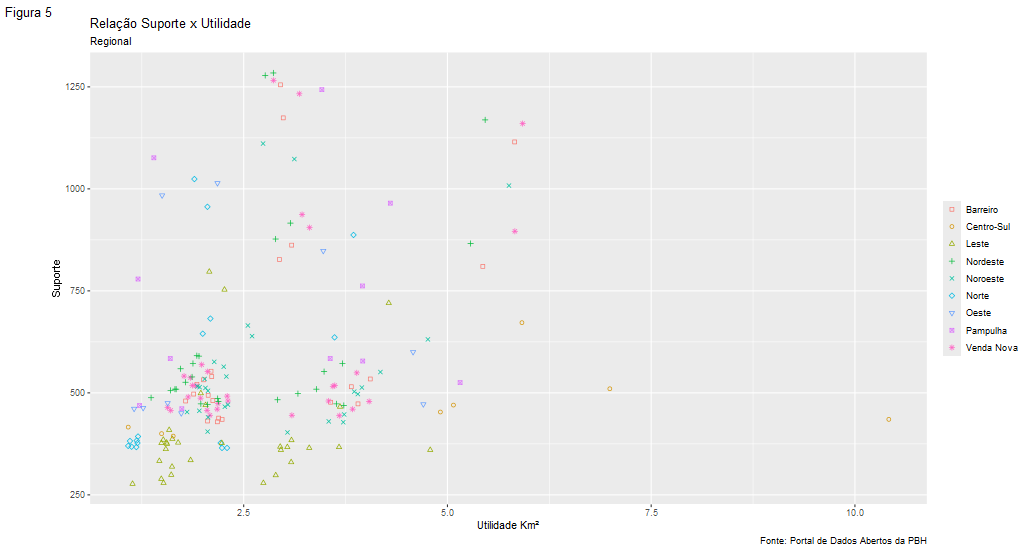
\includegraphics[scale=0.35]{imagens/utilidade_suporte.png}
            \end{figure}
\end{frame}

\subsection{Utilidade negativa m²}
\begin{frame}

    \begin{itemize}
    
        \item As regionais Pampulha e Norte tiveram um impacto negativo em lotes vagos, indicando áreas vagas proximas a terrenos com construção.
    \end{itemize}
\end{frame}

\subsection{Descoberta de Subgrupo - Alvo Padrão de Acabamento P5}
\begin{frame}

    \begin{figure}[!htbp]
                \centering
       	    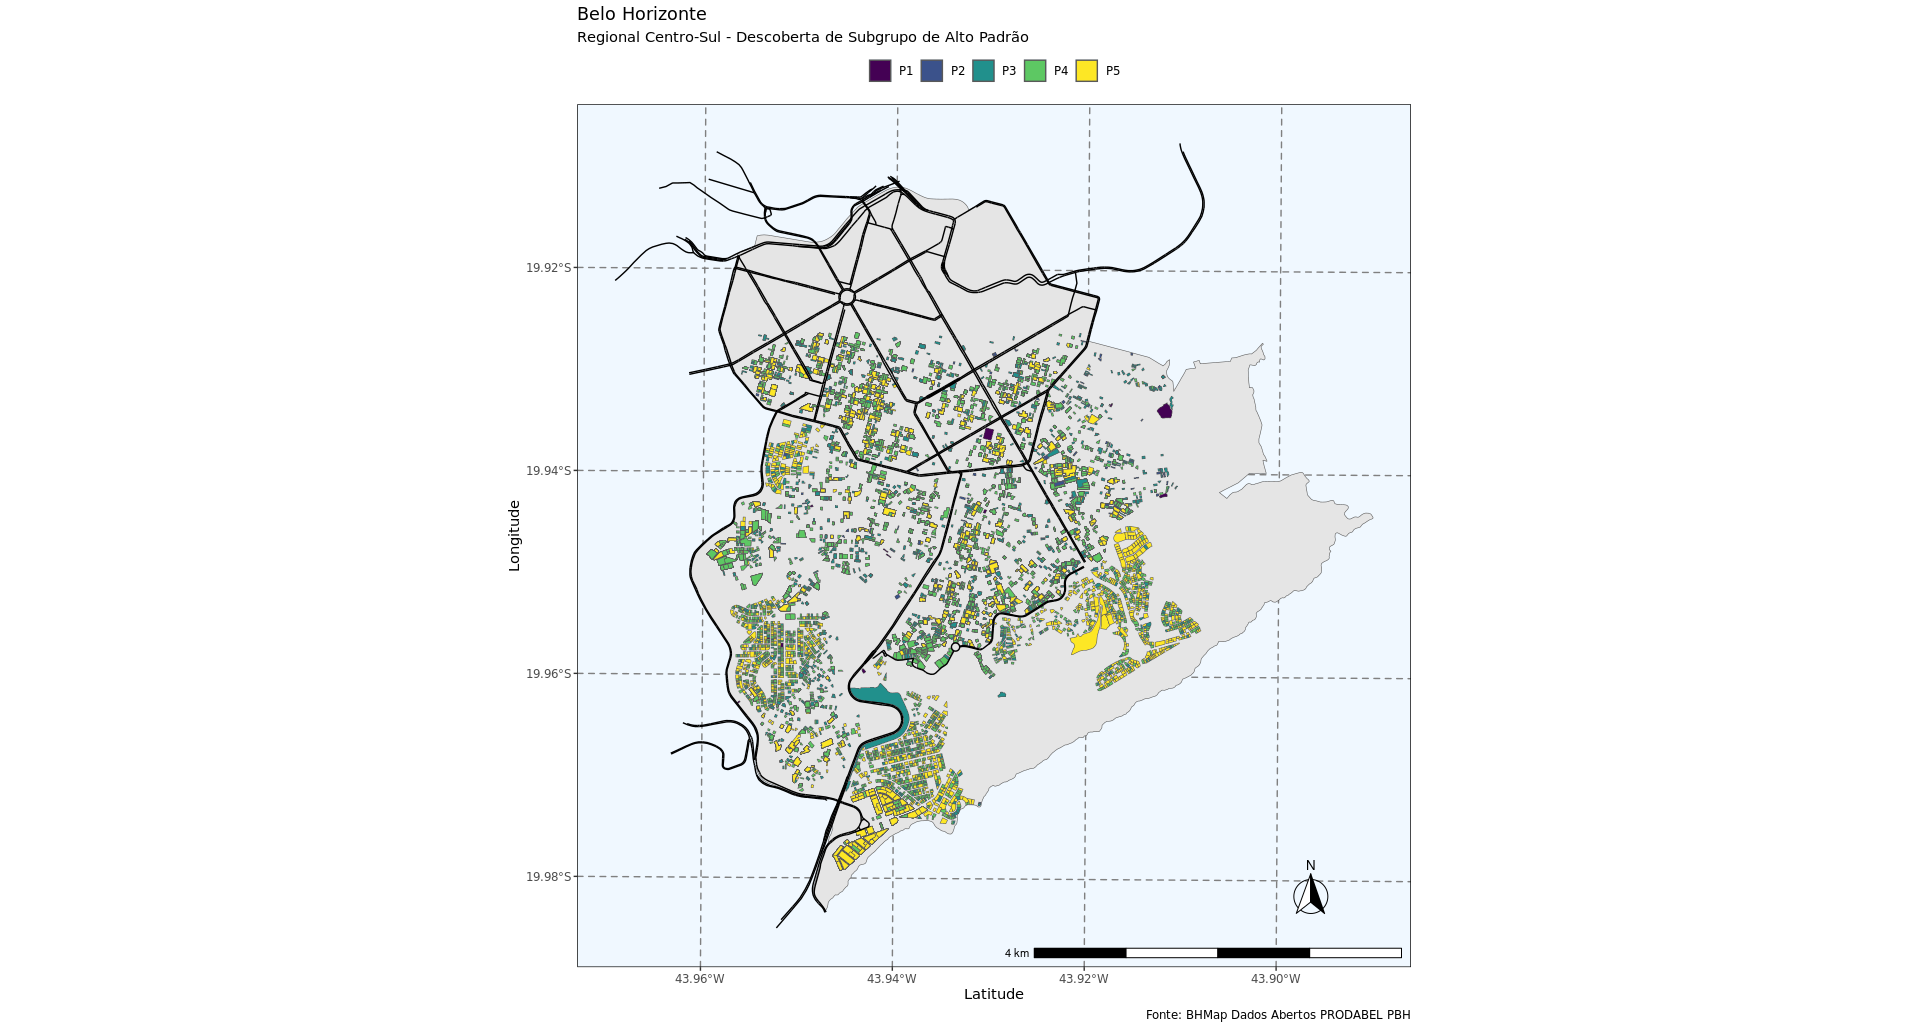
\includegraphics[scale=0.26]{imagens/cortana3.png}
            \end{figure}
\end{frame}

\subsection{Descoberta de Subgrupo - Alvo Tipo Construtivo Apartamento}
\begin{frame}

    \begin{figure}[!htbp]
                \centering
       	    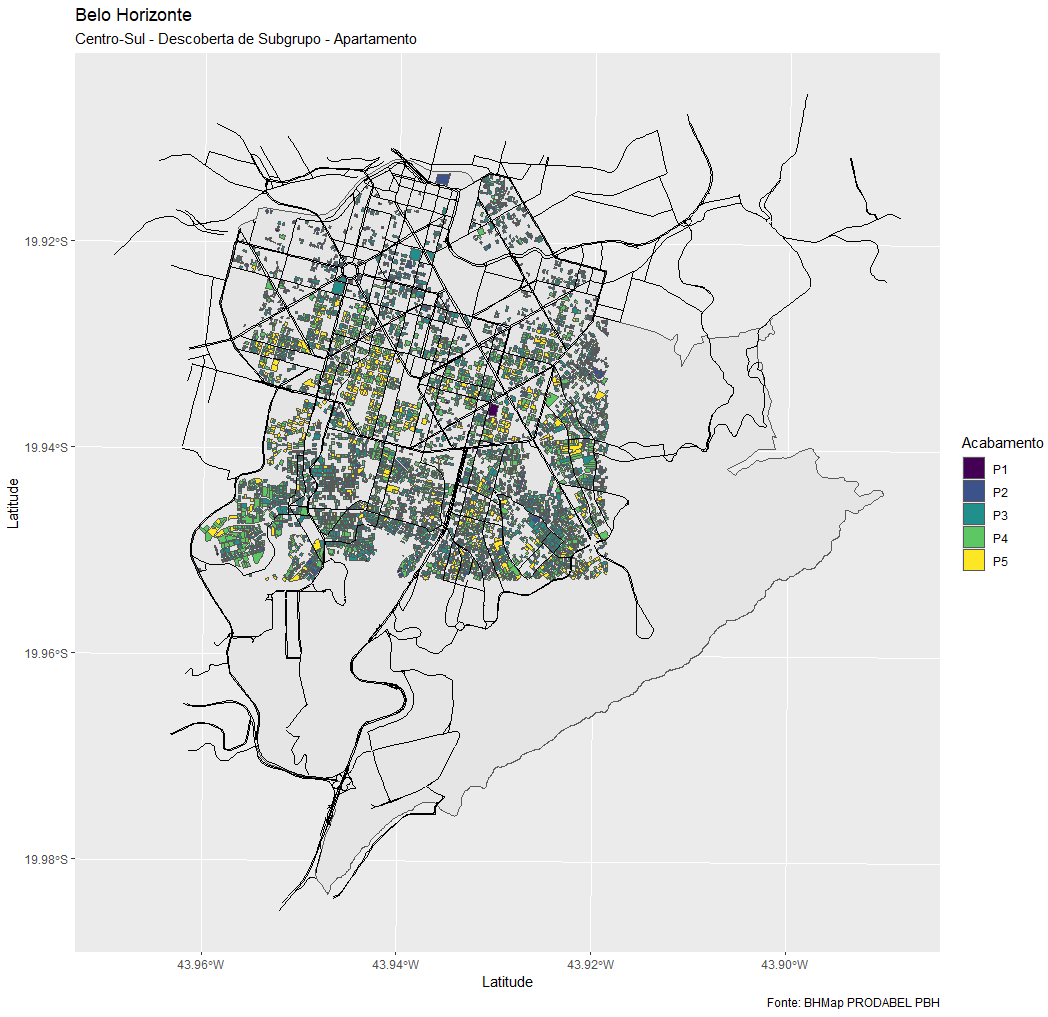
\includegraphics[scale=0.26]{imagens/cortana-ap.png}
            \end{figure}
\end{frame}

\subsection{Descoberta de Subgrupo - Gentrificação}
\begin{frame}

	\begin{table}[]
		\begin{tabular}{|l|l|}
			\hline
			\textbf{Zona Homogenia} & \textbf{Núcleos Familiáres}\\
			\hline
			\hline
			CS407 & 10 \\
			\hline
			CS313 & 12 \\
			\hline
			CS210, CS212 & 13 \\
			\hline
			CS411 & 23 \\
			\hline
		\end{tabular}
	\end{table}
\end{frame}
\subsection{Gentrificação}
\begin{frame}

    \begin{figure}[!htbp]
                \centering
       	    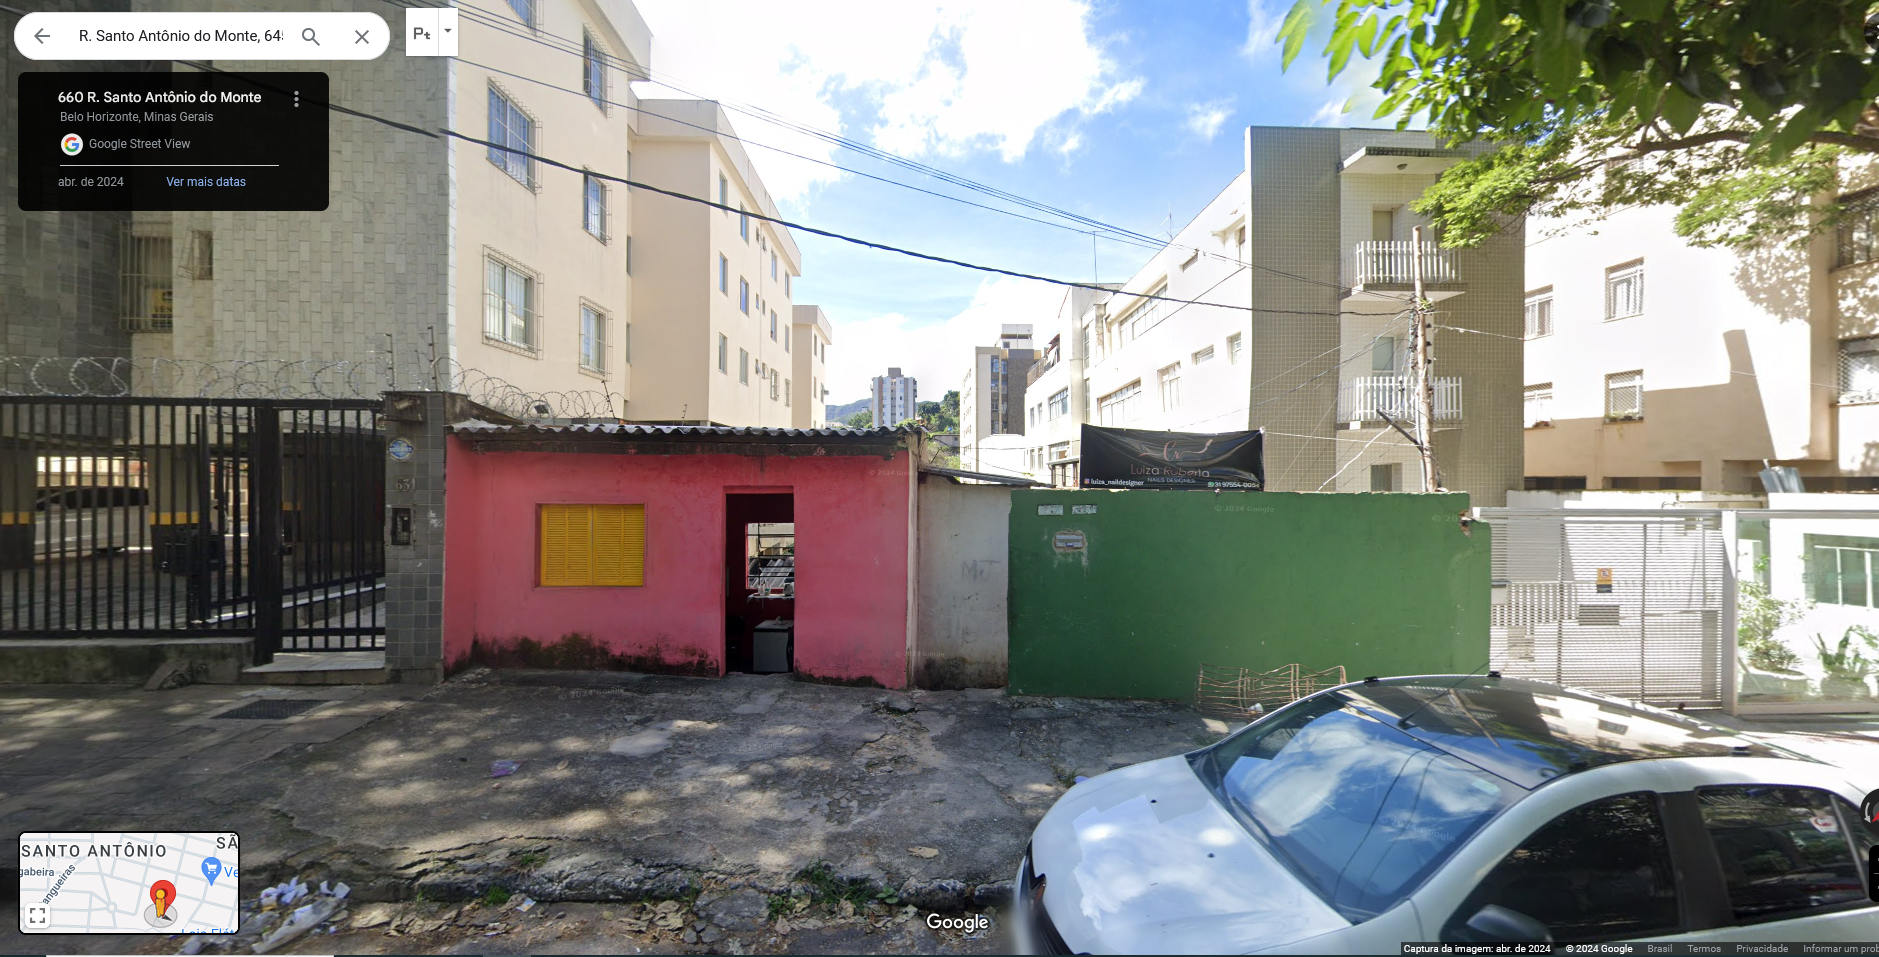
\includegraphics[scale=0.26]{imagens/gentrificacao.png}
            \end{figure}
\end{frame}


